\chapter{DESENVOLVIMENTO}

\section{Circuito retificador em ponte}

\begin{figure}[H]
    \centering
    \fbox{
        \parbox{0.975\textwidth}{
            \centering
            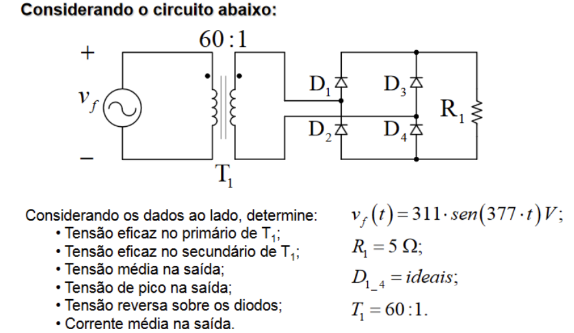
\includegraphics[]{images/circuito_slide_01.png}
        }}
    \caption{Circuito 01}
    \vspace{-0.3cm}
    \label{fig:Circuito01}
\end{figure}

Considerando o circuito da figura \ref{fig:Circuito01}, temos que:

\begin{Resolucao}[H]
    \fbox{
        \parbox{0.975\textwidth}{
            \vspace{0.40cm}
            \centering
            \[Vp = \textcolor{red}{311V}\]
            \[n = \frac{1}{60} = \textcolor{red}{0.0166\dots}\]
            \[Vpico = Vp * n \]

            \[\textnormal{Tensão eficaz no primário de T1: } \frac{311}{\sqrt[2]{2}} = \textcolor{red}{220V}\]
            \[\textnormal{Tensão eficaz no secundário de T1: } \frac{Eficaz1}{Fator} \rightarrow \frac{220}{60} = \textcolor{red}{3.67V} \]
            \[\textnormal{Tensão de pico de entrada no secundário: } Vpico = \frac{311}{60} \simeq \textcolor{red}{5.18V}\]
            \[\textnormal{Tensão média na saída: }  \frac{Vpico - (0.7 * 2)}{\pi} * 2 \simeq \textcolor{red}{2.41V}\]
            \[\textnormal{Tensão de pico na saída: } Vpico - (0.7 * 2) = \textcolor{red}{3,79V}\]
            \[\textnormal{Tensão reversa sobre o diodo: } \textcolor{red}{-4.49V}\]
            \[\textnormal{Corrente média na saída: }  \frac{TensaoMédia}{Ressistencia} \rightarrow \frac{2.41}{5} \simeq \textcolor{red}{0.482A}\]
            \[\textnormal{Corrente de pico no diodo: } \frac{TensãoDePico}{Carga} = \frac{3.79}{5} = \textcolor{red}{0.758A} \]
            \textcolor{red}{\textbf{OBSERVAÇÃO:}} \textcolor{red}{Pode-se observar que a frequência na saída é o dobro, e o período é a metade da entrada.}

            
            % \[\textnormal{Tensão de pico de entrada no primeiro: } \textcolor{red}{311V}\]
            % \[N = \textcolor{red}{\frac{1}{60}}\]
            % \[\textnormal{Tensão de pico na entrada do secundário: } Vf * n * \frac{1}{60} = \textcolor{red}{5.18V}\]
            % \[\textnormal{Tensão de pico na saída: } 5.18 - 1.4 = \textcolor{red}{3.78V}\]
        }
    }
    \captionof*{Resolucao}{Resolução: Circuito Exercício 1}
    \label{res:circuito01}
\end{Resolucao}

\begin{figure}[H]
    \centering
    \fbox{
        \parbox{0.975\textwidth}{
            \centering
            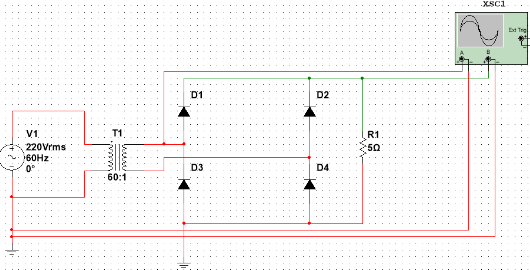
\includegraphics[]{images/simulacoes/circuito_01.png}
        }}
    \caption{Simulação: Circuito 01}
    \vspace{-0.3cm}
    \label{fig:SimulacaoCircuito01}
\end{figure}

\begin{figure}[H]
    \centering
    \fbox{
        \parbox{0.975\textwidth}{
            \centering
            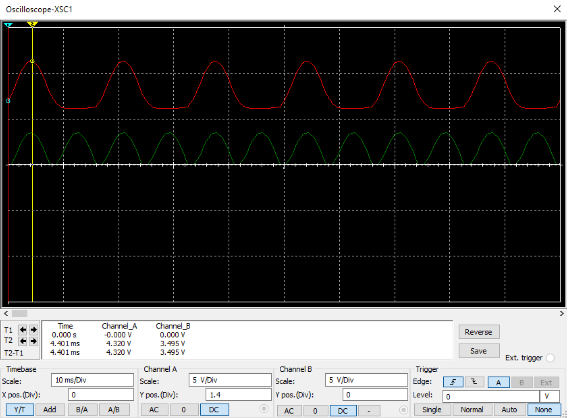
\includegraphics[width=0.975\textwidth]{images/simulacoes/osciloscopio_circuito01.png}
        }}
    \caption{Osciloscópio: Circuito 01}
    \vspace{-0.3cm}
    \label{fig:OsciloscopioCircuito01}
\end{figure}

Com a tabela \ref{tab:Comparacao1Circuito} podemos comparar os resultados obtidos por simulação com os resultados obtidos por cálculo, na qual comprovam que os cálculos estavam corretos.

\begin{quadro}[H]
    \centering
    \caption{Comparação entre os resultados obtidos por simulação e os resultados obtidos por cálculo do circuito 01}
    \begin{tabular}{|C{0.19\textwidth}|C{0.24\textwidth}|C{0.24\textwidth}|C{0.24\textwidth}|C{0.24\textwidth}|}
        \hline
        \rowcolor[HTML]{C0C0C0}
        \textbf{Modelo\textbackslash{}Variáveis} & \textbf{Tensão de pico de entrada no 2} & \textbf{Tensão de pico de saída no 2} \\
        \hline
        Calculado & 5.18V & 3.78V \\
        \hline
        Simulado & 4.401V & 3.495V \\
        \hline
    \end{tabular}
    \vspace{-0.6cm}
    \label{tab:Comparacao1Circuito}
\end{quadro}

O objetivo da ponte retificadora é usar uma ponte de diodos para que em cada semiciclo da fonte, 2 diodos começaram a conduzir, gerando cada par uma onda, onde juntos formam uma onda completa. Cada diodo tem uma queda de tensão de 0,7v.

\section{Retificador de meia onda com filtro capacitivo}

\begin{figure}[H]
    \centering
    \fbox{
        \parbox{0.975\textwidth}{
            \centering
            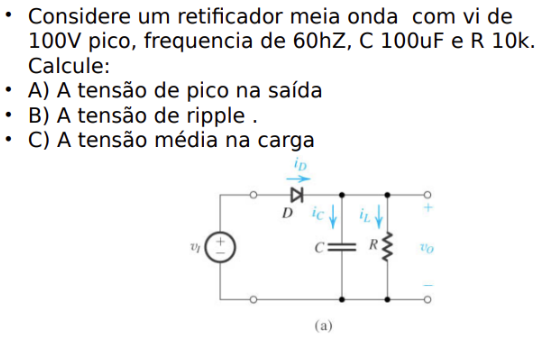
\includegraphics[]{images/circuito_slide_02.png}
        }}
    \caption{Circuito 02}
    \vspace{-0.3cm}
    \label{fig:Circuito02}
\end{figure}

Considerando o circuito da figura \ref{fig:Circuito02}, temos que:

\begin{Resolucao}[H]
    \fbox{
        \parbox{0.975\textwidth}{
            \vspace{0.40cm}
            \centering
            \[\textnormal{Tensão de pico na saída: } Vi - 0.7V \rightarrow 100-0.7 = \textcolor{red}{99.3V}\]
            \[\textnormal{A tensão de ripple: } Vr = \frac{vp}{Frc} \rightarrow \frac{99.3}{60*100K*100u} = \textcolor{red}{1.655V}\]
            \[\textnormal{A tensão média na carga: } Vdc = Vp - \frac{vr}{2} \rightarrow 99.3 - 0.8275 = \textcolor{red}{98.473V}\]
            \[Vrms = \frac{100}{\sqrt[2]{2}} = \textcolor{red}{70.7106}\]
        }
    }
    \captionof*{Resolucao}{Resolução: Circuito Exercício 2}
    \label{res:circuito02}
\end{Resolucao}

\begin{figure}[H]
    \centering
    \fbox{
        \parbox{0.975\textwidth}{
            \centering
            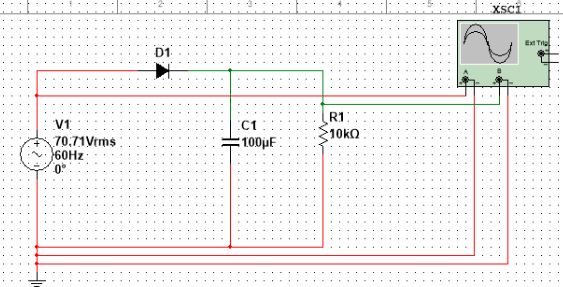
\includegraphics[]{images/simulacoes/circuito_02.png}
        }}
    \caption{Simulação: Circuito 02}
    \vspace{-0.3cm}
    \label{fig:SimulacaoCircuito02}
\end{figure}

\begin{figure}[H]
    \centering
    \fbox{
        \parbox{0.975\textwidth}{
            \centering
            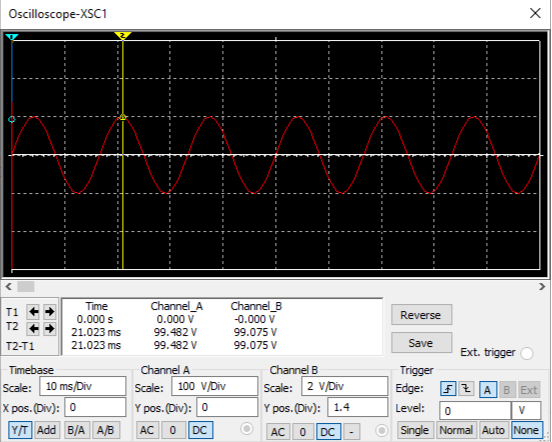
\includegraphics[width=0.975\textwidth]{images/simulacoes/osciloscopio_circuito02.png}
        }}
    \caption{Osciloscópio: Circuito 02}
    \vspace{-0.3cm}
    \label{fig:OsciloscopioCircuito02}
\end{figure}

\begin{figure}[H]
    \centering
    \fbox{
        \parbox{0.975\textwidth}{
            \centering
            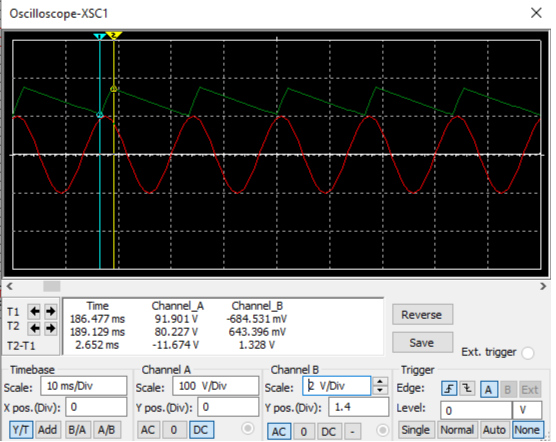
\includegraphics[width=0.975\textwidth]{images/simulacoes/osciloscopio_circuito02_ripple.png}
        }}
    \caption{Osciloscópio: Circuito 02 - Ripple}
    \vspace{-0.3cm}
    \label{fig:OsciloscopioCircuito02Ripple}
\end{figure}

A forma de onda da tensão de ripple, é a diferença entre os dois ponteiros do osciloscópio, que é a diferença entre os dois semiciclos da onda de entrada, onde o primeiro ponteiro é a tensão de pico de entrada e o segundo ponteiro é a tensão de pico de saída. A imagem \ref{fig:OsciloscopioCircuito02Ripple} mostra a tensão de ripple.

Com a tabela \ref{tab:Comparacao2Circuito} podemos comparar os resultados obtidos por simulação com os resultados obtidos por cálculo, na qual comprovam que os cálculos estavam corretos.

\begin{quadro}[H]
    \centering
    \caption{Comparação entre os resultados obtidos por simulação e os resultados obtidos por cálculo do circuito 02}
    \begin{tabular}{|C{0.19\textwidth}|C{0.24\textwidth}|C{0.24\textwidth}|C{0.24\textwidth}|C{0.24\textwidth}|}
        \hline
        \rowcolor[HTML]{C0C0C0}
        \textbf{Modelo\textbackslash{}Variáveis} & \textbf{Tensão de pico de entrada} & \textbf{Tensão saída} & \textbf{Tensão de ripple}\\
        \hline
        Calculado & 100V & 99.3V & 1.65V \\
        \hline
        Simulado & 99.482V & 99.075V & 1.328V \\
        \hline
    \end{tabular}
    \vspace{-0.6cm}
    \label{tab:Comparacao2Circuito}
\end{quadro}

Analisando a forma de onda de tensão de saída do filtro capacitivo, o capacitor descarrega durante o período em que a fonte alimenta o circuito com valor menor de tensão do que o capacitor possui, podemos ver a descarga do capacitor, quando a fonte atinge novamente o valor de tensão maior que a carga contida no capacitor, o capacitor começa a se carregar novamente.

\section{Retificador em ponte com filtro capacitivo}

\begin{figure}[H]
    \centering
    \fbox{
        \parbox{0.975\textwidth}{
            \centering
            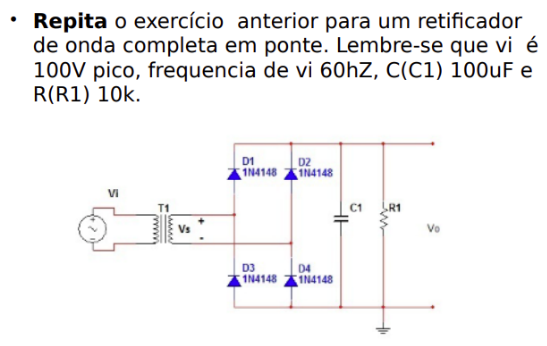
\includegraphics[]{images/circuito_slide_03.png}
        }}
    \caption{Circuito 03}
    \vspace{-0.3cm}
    \label{fig:Circuito03}
\end{figure}

Considerando o circuito da figura \ref{fig:Circuito03}, temos que:

\begin{Resolucao}[H]
    \fbox{
        \parbox{0.975\textwidth}{
            \vspace{0.40cm}
            \centering
            \[\textnormal{Tensão de pico na saída: } Vi - 1.4V \rightarrow 100 - 1.4 = \textcolor{red}{98.6V}\]
            \[\textnormal{Tensão de ripple: } Vr = \frac{Vp}{Frc} \rightarrow \frac{98.6}{120*10K*100u} = \textcolor{red}{0.8216V}\]
            \[\textnormal{Tensão média na carga: } Vp(saida) - \frac{Vr}{2} \rightarrow 98.6 - \frac{0.8216}{2} = \textcolor{red}{98.189V}\]
            \[Vrms = \frac{100}{\sqrt[2]{2}} \simeq \textcolor{red}{70.7106V}\]
        }
    }
    \captionof*{Resolucao}{Resolução: Circuito Exercício 3}
    \label{res:circuito03}
\end{Resolucao}

\begin{figure}[H]
    \centering
    \fbox{
        \parbox{0.975\textwidth}{
            \centering
            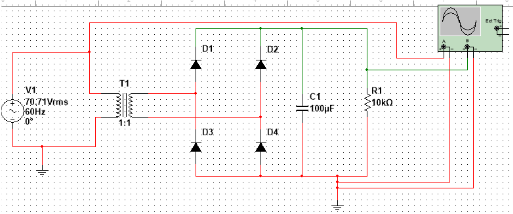
\includegraphics[]{images/simulacoes/circuito_03.png}
        }}
    \caption{Simulação: Circuito 03}
    \vspace{-0.3cm}
    \label{fig:SimulacaoCircuito03}
\end{figure}

\begin{figure}[H]
    \centering
    \fbox{
        \parbox{0.975\textwidth}{
            \centering
            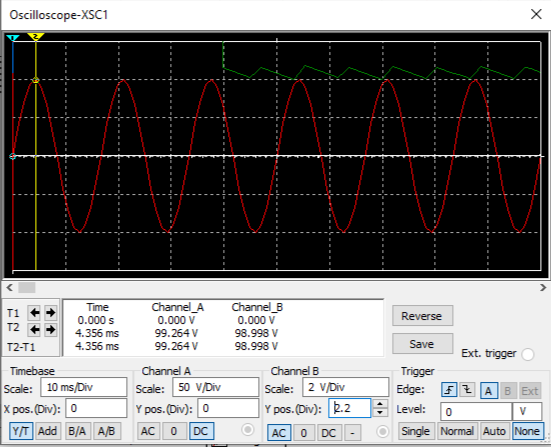
\includegraphics[width=0.975\textwidth]{images/simulacoes/osciloscopio_circuito03.png}
        }}
    \caption{Osciloscópio: Circuito 03}
    \vspace{-0.3cm}
    \label{fig:OsciloscopioCircuito03}
\end{figure}

\begin{figure}[H]
    \centering
    \fbox{
        \parbox{0.975\textwidth}{
            \centering
            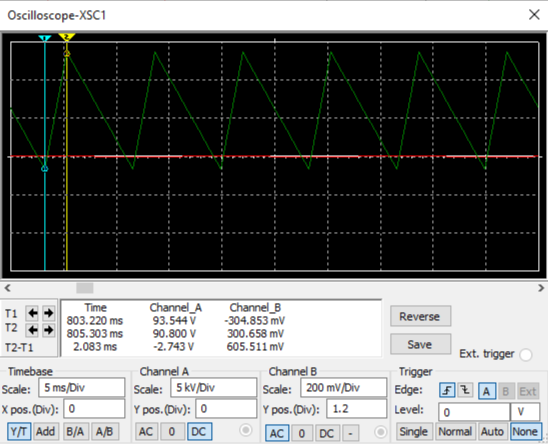
\includegraphics[width=0.975\textwidth]{images/simulacoes/osciloscopio_circuito03_ripple.png}
        }}
    \caption{Osciloscópio: Circuito 03 - Ripple}
    \vspace{-0.3cm}
    \label{fig:OsciloscopioCircuito03Ripple}
\end{figure}

Com a tabela \ref{tab:Comparacao3Circuito} podemos comparar os resultados obtidos por simulação com os resultados obtidos por cálculo, na qual comprovam que os cálculos estavam corretos.

\begin{quadro}[H]
    \centering
    \caption{Comparação entre os resultados obtidos por simulação e os resultados obtidos por cálculo do circuito 03}
    \begin{tabular}{|C{0.19\textwidth}|C{0.24\textwidth}|C{0.24\textwidth}|C{0.24\textwidth}|C{0.24\textwidth}|}
        \hline
        \rowcolor[HTML]{C0C0C0}
        \textbf{Modelo\textbackslash{}Variáveis} & \textbf{Tensão de pico de entrada} & \textbf{Tensão saída} & \textbf{Tensão de ripple}\\
        \hline
        Calculado & 100V & 98.6V & 0.8216V \\
        \hline
        Simulado & 99.264V & 98.998V & 0.605V \\
        \hline
    \end{tabular}
    \vspace{-0.6cm}
    \label{tab:Comparacao3Circuito}
\end{quadro}

Avaliando então percebermos que a frequência de saída do circuito é o dobro da frequência do sinal de entrada.